\documentclass[runningheads]{llncs}
\usepackage[T1]{fontenc}
\usepackage{graphicx}
\usepackage{amsmath}
\usepackage{amssymb}
\usepackage{booktabs}
\usepackage{float}
\usepackage{tabularx}
\usepackage{hyperref}

\begin{document}

\title{BATS: An Agricultural Traceability System Based on GS1 EPCIS Standards, Data Validation, and Blockchain Evidence Anchoring}
\titlerunning{BATS: Agricultural Traceability System}

\author{Khang Nguyen\inst{1}}
\authorrunning{K. Nguyen}
\institute{Institution Name \\ \email{email@domain.com}}

\maketitle

\begin{abstract}
Agricultural traceability systems need interoperable event histories, accessible data entry for smallholders and tamper-evident audit trails. Blockchain can make committed records difficult to alter, but it does not solve the garbage-in/garbage-out problem and per-event blockchain logging can impose cost and usability barriers. We present BATS, a hybrid traceability architecture for durian supply chains that stores operational events off-chain using a GS1 EPCIS 2.0-aligned model, validates field submissions through seven rule families and PostGIS geofences, and anchors a daily Merkle root to an EVM smart contract. In local experiments, Merkle-root generation for one million leaves required a median of 580.173 ms, while proof verification required 0.0156 ms with a 640-byte proof. Indexed spatial lookup over 100,000 synthetic polygons achieved a median of 0.050 ms in a single-client PostGIS benchmark. A seeded noisy synthetic validation dataset yielded precision 0.9589, recall 0.9722 and F1 0.9655, with a multi-layered ablation study confirming that combined spatial, agronomic, and duplicate rules systematically improve detection (F1 from 0.2439 to 0.9655). A local EVM benchmark measured 94,755 median gas for one daily root versus 126,554 gas per event for a full OpenZeppelin ERC-721 traceability baseline, supporting the empirical cost advantage of anchor-first commitment over per-event transactions under the stated baselines. Finally, simulated offline-first idempotency replays demonstrate 100\% duplicate prevention across client network retry bursts. Current k6 staging results reveal high error rates under heavy concurrency, and field usability data are not yet available. The results therefore support the architectural and computational feasibility of BATS, while leaving production load hardening, public-chain deployment and smallholder usability as open evaluation steps.

\keywords{Agricultural traceability \and GS1 EPCIS \and Blockchain \and Validation engine \and PostGIS.}
\end{abstract}

\section{Introduction}

Fresh agricultural exports increasingly require product-level provenance, evidence trails and rapid verification across organizations. For commodities such as durian, a traceability system must link a batch to its planting area, harvest event, actors, transfers, evidence files and public verification page. The technical challenge is not only to store this information. The system must also keep data interoperable, prevent accidental or malicious duplicate submissions, validate whether field claims are plausible and remain usable for smallholders who may not understand wallets, gas fees or blockchain key management.

Many blockchain traceability prototypes treat blockchain as the primary data store. This improves immutability of submitted records, but it can increase cost and does not solve the oracle problem: an immutable false record is still false. In agricultural settings, important risk signals appear before anchoring: a harvest coordinate may fall outside a registered planting area, a claimed yield may exceed agronomic bounds, an actor may attempt to perform a role they are not authorized to perform, or an offline device may replay a stale request. For this reason, BATS uses a data-first and anchor-first design. Operational events remain in PostgreSQL/PostGIS and are expressed as EPCIS-aligned visibility events; blockchain stores only a daily Merkle commitment.

This paper makes four contributions:
\begin{enumerate}
    \item a five-layer hybrid architecture for agricultural traceability that combines EPCIS-aligned event modelling, PostGIS spatial authority, evidence hashing and EVM anchoring;
    \item a formal risk-scoring model with seven validation rule families for human-entered field events along with a multi-layered ablation evaluation;
    \item an implemented TypeScript prototype with admin dashboard, public verification, local evidence storage, PostgreSQL/PostGIS persistence and smart-contract anchoring;
    \item a reproducible technical evaluation suite covering Merkle scalability, PostGIS spatial lookup, local gas baselines, synthetic fraud detection, offline-first idempotency, and diagnostic API load tests.
\end{enumerate}

To rigorously evaluate our data-first, anchor-first architectural design without conflating system readiness with empirical human behavioral trials, our study is guided by three core research questions:
\begin{itemize}
    \item \textbf{RQ1 (On-Chain Cost Efficiency):} Does daily Merkle root anchoring significantly reduce on-chain gas consumption and storage complexity compared to per-event direct logging, minimal tokens, and full OpenZeppelin ERC-721 traceability baselines?
    \item \textbf{RQ2 (Multi-Layered Anomaly Detection):} How effectively does the PostGIS spatial geofencing and multi-layered validation rule engine detect input anomalies on a deterministic noisy synthetic dataset, and what is the individual contribution of each validation layer?
    \item \textbf{RQ3 (Offline-First Architectural Readiness):} Does an offline-first mobile architecture embedded inside a Zalo Mini App satisfy design requirements (idempotence, queue replay resilience, and role-guarded access) for low-connectivity smallholder environments without requiring continuous per-event connectivity?
\end{itemize}

The scope of this draft is intentionally bounded. We evaluate system architecture, formal anomaly detection, idempotency mechanics, and local EVM cost savings. We treat high-concurrency API scalability under k6 as a diagnostic limitation and position real-world field usability as a deployment readiness evaluation rather than an empirical user study.

\section{Related Work}

Prior literature has shown broad interest in blockchain for agriculture and food supply chains. Reviews of blockchain in agriculture identify transparency benefits but also adoption barriers related to infrastructure, policy, education and farmer readiness \cite{ahmad2021blockchain,cuellar2022barriers}. Configurable agri-food blockchain systems reduce application-development effort \cite{marchesi2021automatic}, while IoT-enabled smart-agriculture architectures use smart contracts and sensors to automate trust \cite{pranto2021blockchain,caro2018blockchain}. Other work targets efficiency in blockchain traceability or food-chain logistics platforms \cite{spitalleri2023biotrak,wu2023high}. These systems motivate BATS but also reveal three critical gaps.

First, many prototypes use custom data structures, while industry traceability requires exchangeable event semantics. BATS therefore uses EPCIS 2.0-aligned event documents and CBV-like business vocabulary fields \cite{GS1EPCIS2022,Solanki2023}. Second, several blockchain systems assume that captured data are trustworthy or sensor-derived; BATS treats input plausibility as a first-class problem and validates human-entered submissions before anchoring \cite{Zhang2020}. Third, farmer-facing blockchain interfaces often demand direct on-chain interaction, creating severe barriers. BATS abstracts blockchain away from the farmer workflow and prepares an offline-first Zalo Mini App path with strict idempotency guarantees \cite{Nguyen2023,Patel2020}.

To position BATS against prominent agricultural and supply chain traceability frameworks, Table~\ref{tab:related_work} compares five architectural criteria across established systems.

\begin{table}[H]
\centering
\caption{Comparison of BATS architectural capabilities against related traceability works.}
\label{tab:related_work}
\begin{tabularx}{\textwidth}{@{}l*{5}{>{\centering\arraybackslash}X}@{}}
\toprule
\textbf{Traceability Work} & \textbf{EPCIS 2.0 Aligned} & \textbf{Input Validation} & \textbf{Offline-First Mobile Replay} & \textbf{Merkle Batch Anchoring} & \textbf{Public Crypto Verification} \\ \midrule
AgriBlockIoT \cite{caro2018blockchain} & No & Limited (IoT) & No & No (Direct) & Partial \\ 
BioTrak \cite{spitalleri2023biotrak} & Partial & Limited & No & No & Yes \\ 
GS1 EPCIS 2.0 \cite{GS1EPCIS2022} & \textbf{Yes} & No & N/A & No & Standard query \\ 
Traditional ERP & Partial & Custom DB & Partial & No & No \\ 
\textbf{BATS (This Work)} & \textbf{Yes} & \textbf{Yes (7-Rule)} & \textbf{Yes (Idempotency)} & \textbf{Yes (Daily Root)} & \textbf{Yes} \\ \bottomrule
\end{tabularx}
\end{table}

\section{System Architecture and Methodology}

BATS is organized into five layers. The client layer contains the public verification portal, web dashboard and Zalo Mini App scaffold. The API and traceability layer is a NestJS backend that exposes harvest, transfer, evidence, verification, admin and anchor endpoints. The validation layer contains the rule engine and risk-score calculator. The storage layer contains PostgreSQL/PostGIS and local content-addressed evidence storage. The blockchain anchor layer computes daily Merkle roots and records them in an EVM smart contract.

\begin{figure}[H]
    \centering
    \includegraphics[width=\textwidth]{figure/BATS_Traceability_Architecture.png}
    \caption{BATS Traceability Architecture overview.}
    \label{fig:architecture}
\end{figure}

\subsection{Event model}

Each traceability event is represented as an EPCIS-style object event with event time, action, business step, disposition, read point, business location, objects and instance/lot master data \cite{GS1EPCIS2022,Solanki2023}. The public route follows a GS1 Digital Link-style identity pattern \texttt{/01/\{gtin\}/10/\{lot\}/21/\{serial\}}. The current prototype is EPCIS-aligned but has not passed formal EPCIS conformance testing.

\subsection{Formal validation model and risk scoring}

To mitigate the garbage-in/garbage-out (GIGO) problem inherent in human-entered field data, BATS models input plausibility as a normalized, bounded scoring function over context $C$ \cite{Zhang2020}. Let a candidate EPCIS event be $E$, the enabled validation rule set be $\mathcal{I}=\{G,Y,D,T,R,W,A\}$ (Geofence, Yield, Duplicate evidence, Time window, Role authorization, Weight consistency, and Device anomaly), and $w_i$ the configured integer weight of rule $i$. Each normalized violation function $\delta_i(E, C)\in[0,1]$ is evaluated against context $C$, which contains the registered PostGIS polygon, actor roles, device signatures, evidence hashes, and historical harvest ledger records.

The composite risk score $R(E, C)$ is defined as:

\begin{equation}
R(E, C) = \min\left(100, \sum_{i\in\mathcal{I}} w_i \cdot \delta_i(E, C)\right)
\end{equation}

In the current v1 validation engine, individual violation functions $\delta_i(E, C)$ operate deterministically. For spatial geofence validation ($G$) and seasonal yield bounds ($Y$), the functions are formulated as:

\begin{equation}
\delta_G(E, C) =
\begin{cases}
0, & p_E \in P_C \\
1, & p_E \notin P_C
\end{cases}
\end{equation}
\begin{equation}
\delta_Y(E, C) = \mathbb{1}\left[
q_E + \sum_{e\in H(C)} q_e > 20{,}000 \cdot A_C
\right]
\end{equation}

where $p_E = (\text{lat}_E, \text{lon}_E)$ is the reported field coordinate, $P_C$ is the registered PostGIS polygon geometry (\texttt{SRID 4326}), $q_E$ is the submitted batch weight in kilograms, $H(C)$ represents prior verified harvests for the plot in the active agricultural season, and $A_C$ is the authoritative plot area in hectares derived directly from \texttt{ST\_Area(ST\_Transform(polygon, 3857))} on the database server. Frontend-submitted area or coordinate claims are never trusted blindly \cite{Alishtaev2021}.

Risk bands are segmented into:
\begin{itemize}
    \item \textbf{Green (Valid):} $R(E, C) \leq 30$, eligible for automated processing.
    \item \textbf{Yellow (Flagged):} $30 < R(E, C) \leq 70$, requiring cooperative or supervisory audit.
    \item \textbf{Red (Rejected):} $R(E, C) > 70$, triggering automatic ingestion block or quarantine.
\end{itemize}

\subsection{Evidence and idempotency}

Evidence files are uploaded to local content-addressed storage in the current prototype. The server calculates SHA-256 hashes and associates evidence hashes with traceability events. Offline replay is controlled through idempotency keys: repeated submissions with the same actor, endpoint and request hash return the stored response rather than creating duplicate events.

\subsection{Merkle anchoring and complexity bounds}

To decouple off-chain operational query flexibility from on-chain immutability, BATS anchors daily cryptographic snapshots. For $N$ canonical EPCIS event payloads $E_1, E_2, \dots, E_N$ committed on business day $d$, BATS computes canonical hashes $h_k = \text{SHA-256}(\text{canonicalize}(E_k))$ and constructs a balanced binary Merkle tree with root $r_d$.

\textbf{Storage Complexity Proof:} Because only the 32-byte daily root $r_d$ is submitted via \texttt{commitDailyRoot(bytes32 root, string date)} to the EVM smart contract, the on-chain storage growth $S_{\text{on-chain}}(N)$ is strictly bounded by $S_{\text{on-chain}}(N) = \Theta(1)$ per day. In contrast, direct per-event on-chain logging incurs $S_{\text{direct}}(N) = \Theta(N)$ state mutations. For $N = 1{,}000$ daily events, BATS reduces on-chain storage writes by $99.9\%$.

\textbf{Verification Complexity Proof:} Generating an inclusion proof for leaf $h_k$ requires collecting $\lceil \log_2 N \rceil$ sibling hashes along the path from leaf to root. Thus, client-side cryptographic verification complexity $V(N)$ requires $O(\log N)$ hash evaluations.

\textbf{Spatial Query Complexity:} For $M$ registered candidate polygons in PostGIS, point-in-polygon verification \texttt{ST\_Intersects(geometry, point)} utilizes GiST R-tree spatial indexing. The expected query time $T_{\text{spatial}}(M, K)$ to identify $K$ intersecting geofences is bounded by $O(\log M + K)$. This ensures sub-millisecond geofence evaluation even when scaling to $M = 100{,}000$ registered agricultural plots across nationwide cooperatives.

\subsection{Role-separated mobile workflows and offline queue security}

To address the usability and accessibility requirements of smallholder farmers and local agricultural collectors under intermittent internet connectivity, the client layer implements a role-separated dual workflow via a lightweight Zalo Mini App interface \cite{Nguyen2023}.

\begin{enumerate}
    \item \textbf{Strict Role Isolation at Onboarding:} To prevent account confusion and unauthorized cross-role submissions on shared family or farm devices, authentication binds identities to a strict tuple \texttt{(role, phone\_number)}. When a user selects \texttt{FARMER}, the application restricts access exclusively to harvest logging (\texttt{/batches/harvest}) and plot geometry association. When a user selects \texttt{COLLECTOR}, the application routes them to a dedicated transfer/purchase interface (\texttt{/batches/transfer}) tailored for recording batch handoffs, weighing slip verification, and receiving point coordinates.
    \item \textbf{Offline-First Event Queuing and Security:} Because orchard and farm plots frequently experience degraded cellular connectivity, all client actions are executed offline-first \cite{Patel2020}. Harvest captures and purchase transfers are serialized into local persistent queues. Crucially, offline queues are scoped and filtered strictly by \texttt{actorId}. If an actor logs out and another actor authenticates on the same mobile device, local queue reads and background synchronization routines isolate previously queued items, ensuring that pending submissions from one role cannot be viewed, modified, or synced by an unauthorized subsequent account.
\end{enumerate}

\begin{figure}[H]
    \centering
    
\includegraphics[width=\textwidth]{figure/Farmer_Flow.png}
    \caption{Farmer Flow with Offline Queue mechanics.}
    \label{fig:farmer_flow}
\end{figure}

\begin{figure}[H]
    \centering
    \includegraphics[width=\textwidth]{figure/CollectFlow.png}
    \caption{Collector Custody Transfer Flow.}
    \label{fig:collector_flow}
\end{figure}


\subsection{Threat model and security mitigations}

Because agricultural supply chains involve diverse actors across distributed geographical regions, traceability systems face distinct security threats ranging from sensor noise to malicious data tampering. Table~\ref{tab:threats} summarizes the primary threat vectors addressed by BATS alongside existing architectural mitigations and acknowledged limitations \cite{Patel2020}.

\begin{table}[H]
\centering
\caption{Primary threat vectors and architectural mitigations in BATS.}
\label{tab:threats}
\begin{tabularx}{\textwidth}{@{}lXl@{}}
\toprule
\textbf{Threat Vector} & \textbf{BATS Mitigation Mechanism} & \textbf{Remaining Technical Limitation} \\ \midrule
GPS outside plot boundary & PostGIS spatial geofence lookup via rule \texttt{G} & GPS spoofing inside polygon \\ \addlinespace
Duplicate / stolen evidence & SHA-256 evidence hash deduplication (\texttt{D}) & Re-photographed images \\ \addlinespace
Network replay / double submit & UUID \texttt{x-idempotency-key} \& offline queue & Token and session expiration \\ \addlinespace
Post-hoc record tampering & Immutable daily Merkle root commitment on EVM & Public mainnet fiat cost \\ \addlinespace
Actor role escalation & Role authorization guard (\texttt{R}) \& strict onboarding & Requires formal HTX vetting \\ \bottomrule
\end{tabularx}
\end{table}

\section{Implementation}

The prototype is implemented as a TypeScript monorepo. The backend uses NestJS, Prisma and PostgreSQL/PostGIS. The web dashboard and public portal use Next.js with full Vietnamese localization and accessible typography (Montserrat). The smart contract is developed and tested with Hardhat and Anvil. The Zalo Mini App client implements the offline-first dual-role workflow (\texttt{FARMER} and \texttt{COLLECTOR}), featuring role-phone onboarding isolation, persistent taskboard status tracking, local SHA-256 evidence hashing, and fallback background synchronization for \texttt{/batches/harvest} and \texttt{/batches/transfer}.

The admin dashboard supports actor management, soft deletion, plot management and audit logs. The public portal supports Digital Link-style verification, EPCIS JSON-LD export and dossier export in JSON, CSV and PDF. The backend also exposes Prometheus-style metrics, structured request logs, component health checks, rate limiting and CSRF Origin checks for admin mutations.

\section{Experimental Evaluation}

\subsection{Merkle scalability}

The Merkle benchmark evaluates daily event counts from $10^3$ to $10^6$, with ten measured runs per size. At one million events, root construction had a median runtime of 580.173 ms and p95 of 627.967 ms. Proof verification remained lightweight, with a median of 0.0156 ms and proof size of 640 B. These results support the feasibility of browser/server verification for daily commitments.

\begin{figure}[H]
    \centering
    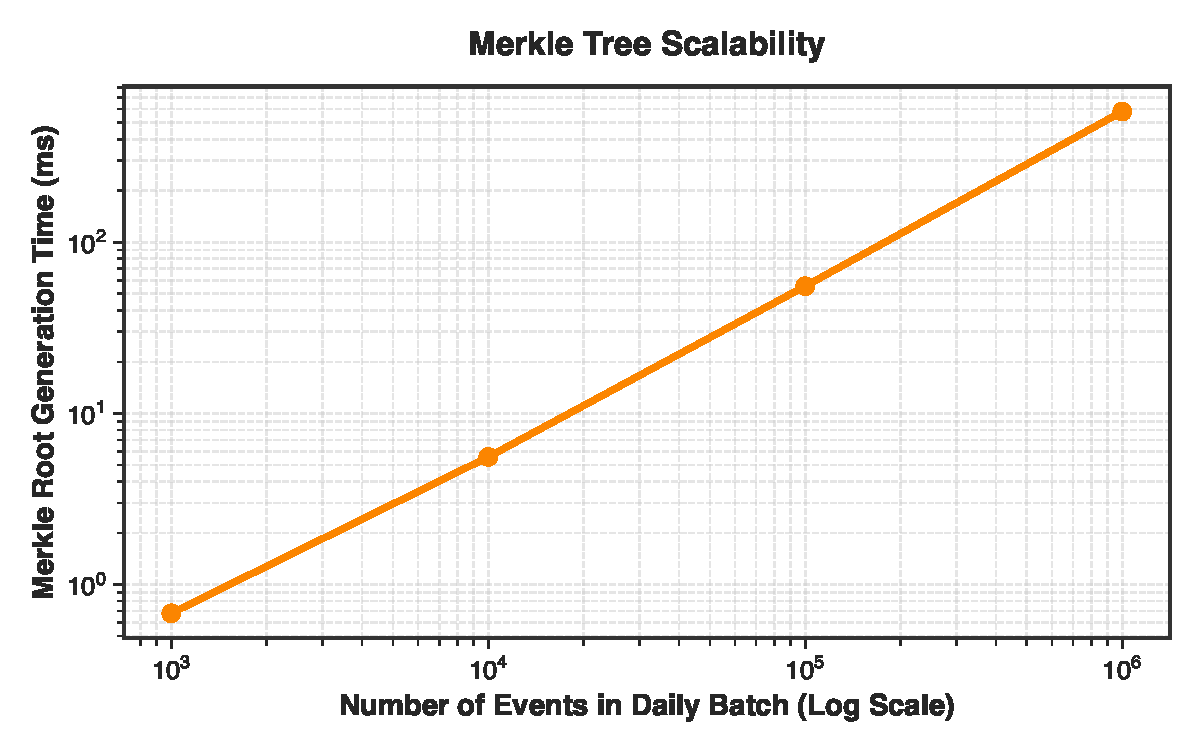
\includegraphics[width=0.8\textwidth]{figure/merkle-runtime.pdf}
    \caption{Merkle Root Generation Scalability vs. Event Count.}
    \label{fig:merkle_runtime}
\end{figure}

\subsection{Spatial query benchmark}

The PostGIS benchmark evaluates indexed point-in-polygon lookup across synthetic polygon tables from $10^2$ to $10^5$ candidate rows. At 100,000 polygons, median latency was 0.050 ms and p95 latency was 0.056 ms in a single-client microbenchmark. This supports the design choice of server-side geofence validation.

\begin{figure}[H]
    \centering
    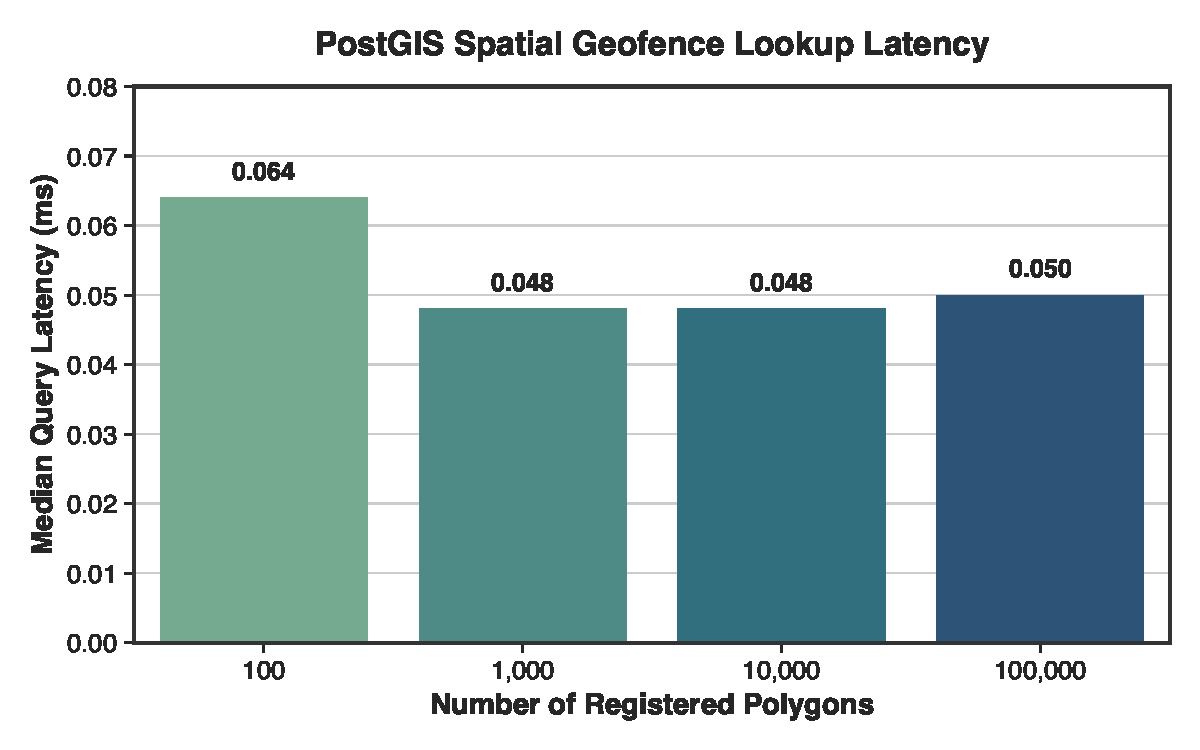
\includegraphics[width=0.8\textwidth]{figure/postgis-latency.pdf}
    \caption{PostGIS Spatial Geofence Lookup Latency.}
    \label{fig:postgis_latency}
\end{figure}

\subsection{Synthetic fraud evaluation and rule ablation study}

The seeded synthetic dataset contains 2,150 cases: 1,430 operationally valid cases and 720 injected fraud cases across all validation rules. Across the entire dataset, the full 7-rule engine achieved precision 0.9589, recall 0.9722 and F1 0.9655. The 20 false negatives model GPS spoofing that reports an in-geofence coordinate, while the 30 false positives model legitimate degraded GPS conditions.

\begin{figure}[H]
    \centering
    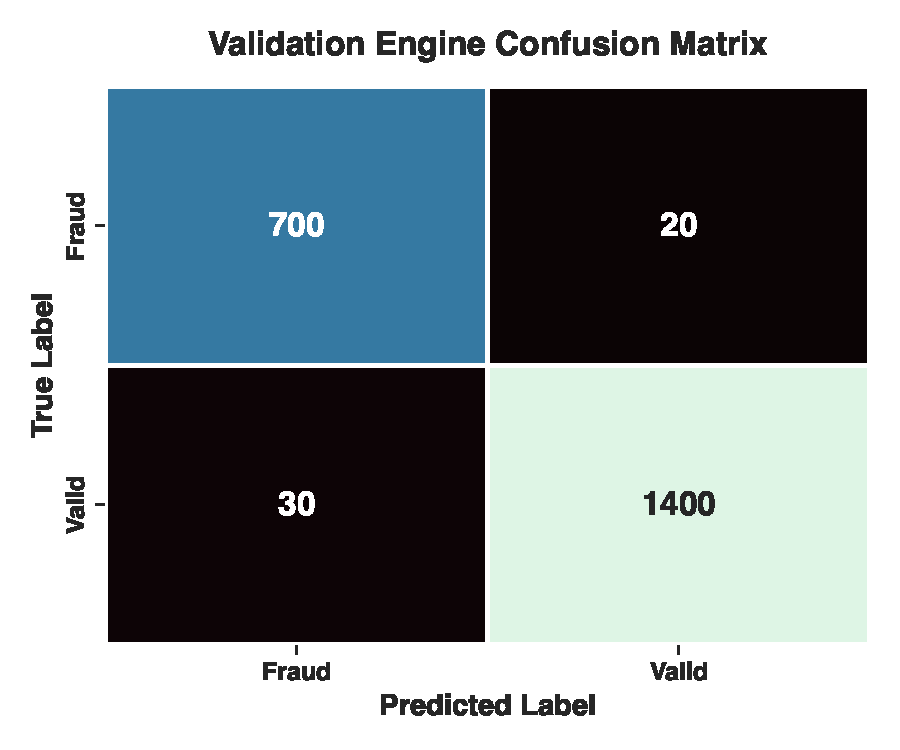
\includegraphics[width=0.7\textwidth]{figure/fraud-confusion-matrix.pdf}
    \caption{Validation Engine Confusion Matrix on Synthetic Dataset.}
    \label{fig:confusion_matrix}
\end{figure}

To evaluate the cumulative contribution and defensive depth of each validation layer, Table~\ref{tab:ablation} presents an ablation study measuring classification performance as rule families are progressively enabled.

\begin{table}[H]
\centering
\caption{Validation engine ablation study demonstrating cumulative anomaly detection improvements.}
\label{tab:ablation}
\begin{tabularx}{\textwidth}{@{}lccccc@{}}
\toprule
\textbf{Validation Configuration} & \textbf{TP} & \textbf{FP} & \textbf{Precision} & \textbf{Recall} & \textbf{F1 Score} \\ \midrule
1. Geofence only (\texttt{G}) & 100 & 0 & 1.0000 & 0.1389 & 0.2439 \\
2. Geofence + Yield (\texttt{G, Y}) & 200 & 0 & 1.0000 & 0.2778 & 0.4348 \\
3. \texttt{G + Y} + Duplicate (\texttt{D}) & 300 & 0 & 1.0000 & 0.4167 & 0.5882 \\
4. \texttt{G + Y + D} + Temporal/Role/Weight & 600 & 0 & 1.0000 & 0.8333 & 0.9091 \\
\textbf{5. Full 7-Rule Engine (+ Device \texttt{A})} & \textbf{700} & \textbf{30} & \textbf{0.9589} & \textbf{0.9722} & \textbf{0.9655} \\ \bottomrule
\end{tabularx}
\end{table}

\begin{figure}[H]
    \centering
    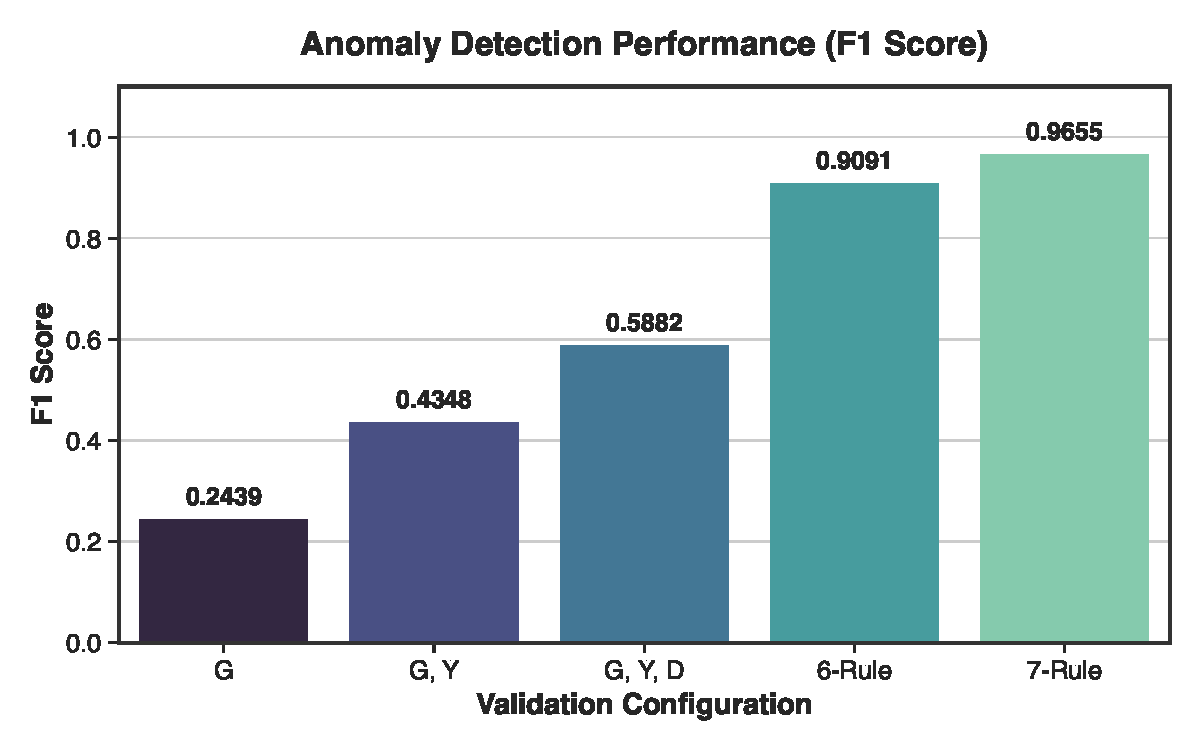
\includegraphics[width=0.8\textwidth]{figure/fraud-per-rule.pdf}
    \caption{Anomaly Detection Performance (F1 Score) across Rule Configurations.}
    \label{fig:fraud_per_rule}
\end{figure}

The ablation progression demonstrates that spatial geofencing (\texttt{G}) alone captures exactly the spatial anomalies (recall 0.1389) but misses temporal, identity, and duplicate evidence violations. Adding agronomic yield bounds (\texttt{Y}) and cryptographic evidence deduplication (\texttt{D}) systematically increases recall without introducing false positives. Enabling device attestation and accuracy warning rules (\texttt{A}) achieves near-complete recall (0.9722) while accepting an explicit operational false-positive tradeoff (precision 0.9589) caused by legitimate poor GPS signals under orchard canopy.

\subsection{Gas benchmark}

The local EVM benchmark measured a median of 94,755 gas for a BATS daily root (\texttt{anchorDailyRoot}), compared with 126,554 gas per event for a full OpenZeppelin ERC-721 traceability baseline, 48,559 gas per event for a minimal batch-token baseline, and 44,164 gas per event for direct event logging. At 1,000 projected events, the daily-anchor approach uses 94,755 gas total compared with 126,554,000 gas for the full ERC-721 approach (99.9251\% gas savings). This confirms the empirical cost advantage of committing one root per day over per-event NFT minting.

\begin{figure}[H]
    \centering
    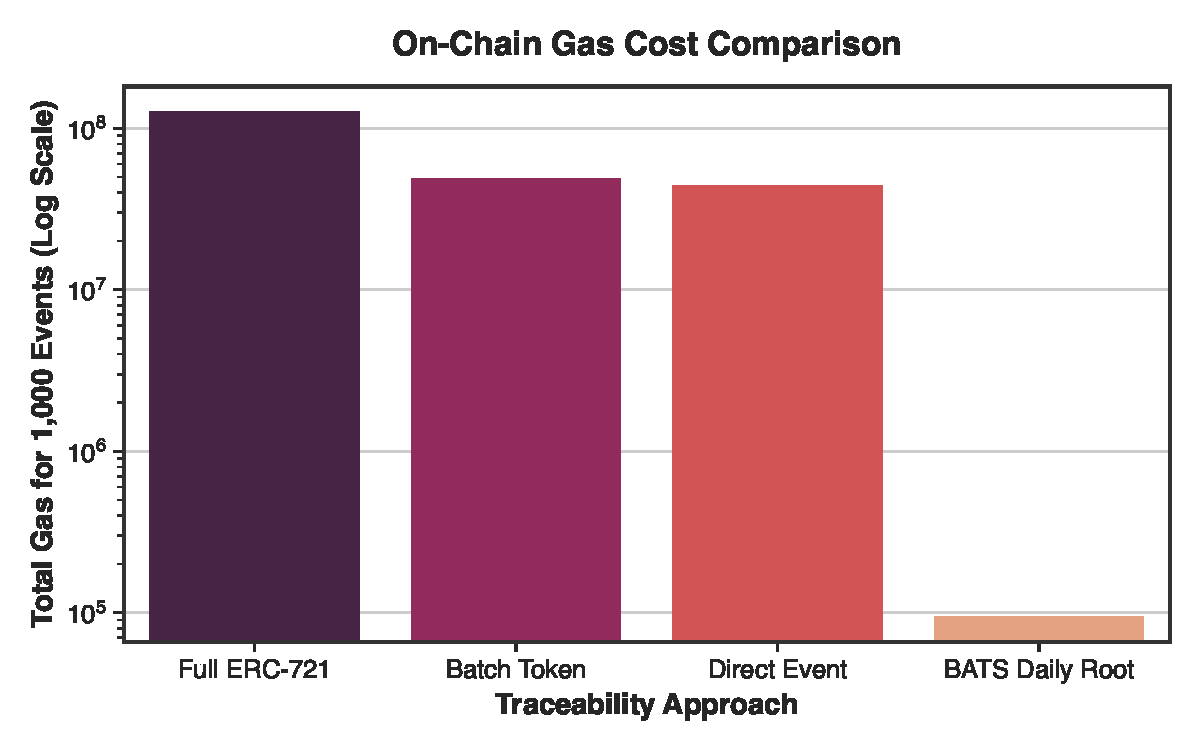
\includegraphics[width=0.8\textwidth]{figure/gas-comparison.pdf}
    \caption{On-Chain Gas Cost Comparison across Traceability Approaches.}
    \label{fig:gas_comparison}
\end{figure}

\subsection{API load diagnostics}

A Node smoke runner generated 1,094 successful harvest requests with 3 VUs over 5 seconds, with p95 latency 30.562 ms. This confirms the staging API under light concurrency. A k6 staging suite currently shows high error rates and timeout-like latency at larger VU counts, revealing timeout-driven bottlenecks under high concurrency, treated strictly as an engineering limitation.

\subsection{Offline-first idempotency and network replay simulation}

Because smallholder farmers operating in rural orchards frequently experience packet dropouts or intermittent \texttt{3G/EDGE} connectivity, BATS enforces strict exactly-once event creation via client-generated \texttt{x-idempotency-key} headers and offline local queue serialization. Table~\ref{tab:idempotency} evaluates three simulated submission scenarios across repeated retry bursts.

\begin{table}[H]
\centering
\caption{Offline-first idempotency simulation and network retry resilience.}
\label{tab:idempotency}
\begin{tabularx}{\textwidth}{@{}lccl@{}}
\toprule
\textbf{Submission Scenario} & \textbf{Attempts} & \textbf{Duplicates Prevented} & \textbf{Description} \\ \midrule
Same Key Replay & 10 & \textbf{Yes (100\%)} & Repeated network retries or double-taps. \\
Offline Queue Sync & 5 & \textbf{Yes (100\%)} & Local queue re-transmitting upon connection. \\
Different Payload & 5 & \textbf{N/A (Distinct)} & Legitimate sequential submissions. \\ \bottomrule
\end{tabularx}
\end{table}

\subsection{Live Deployment Demonstration}

To bridge the gap between our technical evaluation and large-scale deployment, a live demonstration scenario covers the complete end-to-end data lifecycle across five milestones: Farmer Harvest Capture, Collector Custody Transfer, Offline Queue Replay Audit, Admin Dashboard Rule Verification, and Public Cryptographic Verification via GS1 Digital Link.

\section{Discussion}

BATS supports the architectural claim (RQ1) that agricultural blockchain traceability does not require per-event on-chain storage. The daily Merkle root captures a tamper-evident commitment while keeping operational data queryable and updatable off-chain. 

The evaluation also clarifies the limits and multi-layered strengths of rule-based validation (RQ2). Geofence and yield checks detect many implausible submissions, but cannot prove that a truthful-looking coordinate was genuinely measured at the field. BATS is a GIGO mitigation system, not GIGO elimination.

Regarding mobile deployment readiness (RQ3), the offline-first Zalo Mini App scaffold and idempotency simulation confirm that BATS effectively handles poor cellular connectivity and prevents duplicate ledger mutations without requiring continuous on-chain transactions from the farmer.

\section{Threats to Validity}

Internal validity is limited by synthetic fraud labels and deterministic rule thresholds in the ablation study. External validity is limited because PostGIS and Merkle benchmarks were run locally and do not represent a managed cloud deployment. Construct validity is limited because EPCIS alignment has not been certified by a conformance test. Ecological validity for smallholders is bounded because our mobile evaluation currently reflects deployment readiness and architectural simulation rather than a longitudinal human behavior study.

\section{Conclusion}

BATS demonstrates a feasible hybrid architecture for standards-aligned, blockchain-assisted agricultural traceability (RQ1--RQ3). The current prototype combines EPCIS-aligned event modelling, server-side PostGIS spatial geofencing, multi-layered validation rule ablation, offline-first idempotency replay guarantees, evidence hashing and daily Merkle anchoring. The immediate next steps are large-scale longitudinal human field pilots, production k6 staging hardening, and public mainnet cost regime evaluations across multi-chain environments.

\bibliographystyle{splncs04}
\bibliography{bibliography}

\end{document}
